%% FEUP THESIS STYLE for LaTeX2e
%% how to use feupteses (Portuguese version)
%% FEUP, JCL & JCF, October 2024
%%
%% Read the documentation inline and at the included `README` file
%%
%% PLEASE send improvements to jcf at fe.up.pt and to jlopes at fe.up.pt
%%
%% This is the portuguese version of the main file

\documentclass[11pt,a4paper]{report}

%% For two-sided printing (for dead-tree output) comment previous line
%% and uncomment the next line
%\documentclass[11pt,a4paper,twoside,openright]{report}

%% Source text uses in UTF-8 encoding
\usepackage[utf8]{inputenc}

%% The package feupteses.sty may take several options
%% There are options for specific FEUP programmes/degrees
%% When no programme specification is given, a generic thesis format is used
%%
%% option  degree/programme
%% -----------------------------
%% meec    Master's degree in Electrical and Computer Engineering
%% meic    Master's degree in Informatics Engineering and Computation   
%% mem     Master's degree in Mechanical Engineering
%% mesw    Master's degree in Software Engineering
%% mci     Master's degree in Information Science

%% In general, the dissertation goes through several stages
%% 
%% option       stage
%%  -----------------------------
%% (no option)  text is in the preparation stage
%% juri         version for evaluation by committee
%% final        version for final submission (after accpetance)

%% Generic format (for other degrees, including Ph.D. programmes)
\usepackage[portugues]{feupteses} 
%% If you don't use a degree option, you must define the degree below

%% Additional options for feupteses.sty: 
%% - portugues: titles, etc in portuguese
%% - onpaper: links are not shown (for paper versions)
%% - backrefs: include back references from bibliography to citation place
%% - iso: format references according to ISO 690 standard

%% Packages loaded by feupteses.sty
%% url, setspace, makeidx, graphicx, xcolor

%% Include here any other packages you need

%% TIP: use folder ``figures'' to keep all your figures
%% Path to the figures directory
\graphicspath{{figures/}}

%% Change to the appropriate bibliography file
\addbibresource{bibliography.bib}

%%========================================
%% Start of document
%%========================================
\begin{document}

%%----------------------------------------
%% Information about the work
%%----------------------------------------
\title{$<$Dissertation Title$>$}
\author{$<$Author's Full Name$>$}

%% Comment next line if not necessary for degree
\degree{Programa Doutoral em Engenharia Informática}

%% Uncomment next line for date of submission
%\thesisdate{July 31, 2008}

%% Comment next line copyright text if not used
\copyrightnotice{Name of the Author, 2008}

\supervisor{Orientador}{Prof.\ $<$Name of the Supervisor$>$}

%% Uncomment next line if necessary
%\supervisor{Segundo orientador}{Prof.\ $<$Name of the Supervisor$>$}

%% Uncomment committee stuff in the final version if used
%\committeetext{Aprovado em provas públicas pelo Júri:}
%\committeemember{Presidente}{Prof.\ $<$Nome do presidente do júri$>$}
%\committeemember{Arguente}{Prof.\ $<$Nome do arguente do júri$>$}
%\committeemember{Vogal}{Prof.\ $<$Nome do vogal do júri$>$}

%% uncomment next line to draw line for handwritten signature (if necessary)
%\signature

%% Specify cover logo (in folder ``figures'')
\logo{uporto-feup.pdf}

%% Uncomment next line for additional text below the author's name (front page)
%\additionalfronttext{<Additional text>}

%%----------------------------------------
%% Preliminary materials
%%----------------------------------------

% remove unnecessary \include{} commands
\begin{Prolog}
  %% abstract.tex: abstract in PT and EN  (FEUP regulations)
%% -------------------------------------------------------
\chapter*{Resumo}
%
Este documento ilustra o formato a usar em dissertações na Feup.
São dados exemplos de margens, cabeçalhos, títulos, paginação, estilos
de índices, etc. 
São ainda dados exemplos de formatação de citações, figuras e tabelas,
equações, referências cruzadas, lista de referências e índices.
Este documento não pretende exemplificar conteúdos a usar. 
É usado o \emph{Loren Ipsum} para preencher a dissertação.
%
Lorem ipsum dolor sit amet, consectetuer adipiscing elit. Etiam vitae
quam sed mauris auctor porttitor. Mauris porta sem vitae arcu sagittis
facilisis. Proin sodales risus sit amet arcu. Quisque eu pede eu elit
pulvinar porttitor. Maecenas dignissim tincidunt dui. Pellentesque
habitant morbi tristique senectus et netus et malesuada fames ac
turpis egestas. Donec non augue sit amet nulla gravida
rutrum. Vestibulum ante ipsum primis in faucibus orci luctus et
ultrices posuere cubilia Curae; Nunc at nunc. Etiam egestas. 
%
Donec malesuada pede eget nunc. Fusce porttitor felis eget mi mattis
vestibulum. Pellentesque faucibus. Cras adipiscing dolor quis
mi. Quisque sagittis, justo sed dapibus pharetra, lectus velit
tincidunt eros, ac fermentum nulla velit vel sapien. Vestibulum sem
mauris, hendrerit non, feugiat ac, varius ornare, lectus. Praesent
urna tellus, euismod in, hendrerit sit amet, pretium vitae,
nisi. Proin nisl sem, ultrices eget, faucibus a, feugiat non,
purus. Etiam mi tortor, convallis quis, pharetra ut, consectetuer eu,
orci. Vivamus aliquet. Aenean mollis fringilla erat. Vivamus mollis,
purus at pellentesque faucibus, sapien lorem eleifend quam, mollis
luctus mi purus in dui. Maecenas volutpat mauris eu lectus. Morbi vel
risus et dolor bibendum malesuada. Donec feugiat tristique erat. Nam
porta auctor mi. Nulla purus. Nam aliquam. 

\chapter*{Abstract}
%
Here goes the abstract written in English. Should say the same.

Lorem ipsum dolor sit amet, consectetuer adipiscing elit. Sed vehicula
lorem commodo dui. Fusce mollis feugiat elit. Cum sociis natoque
penatibus et magnis dis parturient montes, nascetur ridiculus
mus. Donec eu quam. Aenean consectetuer odio quis nisi. Fusce molestie
metus sed neque. Praesent nulla. Donec quis urna. Pellentesque
hendrerit vulputate nunc. Donec id eros et leo ullamcorper
placerat. Curabitur aliquam tellus et diam. 
%
Ut tortor. Morbi eget elit. Maecenas nec risus. Sed ultricies. Sed
scelerisque libero faucibus sem. Nullam molestie leo quis
tellus. Donec ipsum. Nulla lobortis purus pharetra turpis. Nulla
laoreet, arcu nec hendrerit vulputate, tortor elit eleifend turpis, et
aliquam leo metus in dolor. Praesent sed nulla. Mauris ac augue. Cras
ac orci. Etiam sed urna eget nulla sodales venenatis. Donec faucibus
ante eget dui. Nam magna. Suspendisse sollicitudin est et mi. 
%
Fusce sed ipsum vel velit imperdiet dictum. Sed nisi purus, dapibus
ut, iaculis ac, placerat id, purus. Integer aliquet elementum
libero. Phasellus facilisis leo eget elit. Nullam nisi magna, ornare
at, aliquet et, porta id, odio. Sed volutpat tellus consectetuer
ligula. Phasellus turpis augue, malesuada et, placerat fringilla,
ornare nec, eros. Class aptent taciti sociosqu ad litora torquent per
conubia nostra, per inceptos himenaeos. Vivamus ornare quam nec sem
mattis vulputate. Nullam porta, diam nec porta mollis, orci leo
condimentum sapien, quis venenatis mi dolor a metus. Nullam
mollis. Aenean metus massa, pellentesque sit amet, sagittis eget,
tincidunt in, arcu. Vestibulum porta laoreet tortor. Nullam mollis
elit nec justo. In nulla ligula, pellentesque sit amet, consequat sed,
faucibus id, velit. Fusce purus. Quisque sagittis urna at quam. Ut eu
lacus. Maecenas tortor nibh, ultricies nec, vestibulum varius, egestas
id, sapien. 
%
Donec hendrerit. Vivamus suscipit egestas nibh. In ornare leo ut
massa. Donec nisi nisl, dignissim quis, faucibus a, bibendum ac,
diam. Nam adipiscing hendrerit mi. Morbi ac nulla. Nullam id est ac
nisi consectetuer commodo. Pellentesque aliquam massa sit amet
tellus. Vivamus sodales aliquam leo. 
 % the abstract
  \include{un-sdg}   % United Nations Sustainable Development Goals (SGD)
  \chapter*{Acknowledgements}
%\addcontentsline{toc}{chapter}{Acknowledgements}

Aliquam id dui. Nulla facilisi. Nullam ligula nunc, viverra a, iaculis
at, faucibus quis, sapien. Cum sociis natoque penatibus et magnis dis
parturient montes, nascetur ridiculus mus. Curabitur magna ligula,
ornare luctus, aliquam non, aliquet at, tortor. Donec iaculis nulla
sed eros. Sed felis. Nam lobortis libero. Pellentesque
odio. Suspendisse potenti. Morbi imperdiet rhoncus magna. Morbi
vestibulum interdum turpis. Pellentesque varius. Morbi nulla urna,
euismod in, molestie ac, placerat in, orci. 

Ut convallis. Suspendisse luctus pharetra sem. Sed sit amet mi in diam
luctus suscipit. Nulla facilisi. Integer commodo, turpis et semper
auctor, nisl ligula vestibulum erat, sed tempor lacus nibh at
turpis. Quisque vestibulum pulvinar justo. Class aptent taciti
sociosqu ad litora torquent per conubia nostra, per inceptos
himenaeos. Nam sed tellus vel tortor hendrerit pulvinar.  

Fusce gravida placerat sem. Aenean ipsum diam, pharetra vitae, ornare
et, semper sit amet, nibh. Nam id tellus. Etiam ultrices.  

\vspace{10mm}
\flushleft{$<$O Nome do Autor$>$}
  % the acknowledgments
  %% This section is optional and can be removed
\cleardoublepage
\thispagestyle{plain}

\vspace*{8cm}

\begin{flushright}
   \textsl{``Our greatest glory is not in never falling, but in rising every time we fall''} \\
\vspace*{1.5cm}
    Confucius
\end{flushright}
    % initial quotation if desired
  \cleardoublepage
  %% Uncomment next line for PT
  \renewcommand{\contentsname}{Índice}
  \pdfbookmark[0]{Table of Contents}{contents}
  \tableofcontents
  \cleardoublepage
  \pdfbookmark[0]{List of Figures}{figures}
  \listoffigures
  \cleardoublepage
  \pdfbookmark[0]{List of Tables}{tables}
  \listoftables
  %% Abbreviations are in the `abbrevs.tex' file
  %% Omit if there aren't any
  \chapter*{List of Acronyms}
\chaptermark{LIST OF ACRONYMS}


\begin{acronym}[H.264/SVC]
    \acro{AI}{Artificial Intelligence}
%	\acro{API}{Application Program Interface}
	\acro{APR}{Automatic Program Repair}
	\acro{ASR}{Automatic Software Repair}
        \acro{API}{Application Programming Interface}
%	\acro{AST}{Abstract Syntax Tree}
	\acro{CIA}{Confidentiality, Integrity, and Availability}
	\acro{CGC}{Cyber Grand Challenge}
%	\acro{CRS}{Cyber Reasoning System}
%	\acro{CTF}{Capture the Flag}
	\acro{CPE}{Common Platform Enumeration}
	\acro{CVE}{Common Vulnerabilities and Exposures}
	\acro{CWE}{Common Weakness Enumeration}
	\acro{DARPA}{Defense Advanced Research Projects Agency}
	\acro{FL}{Fault Localization}
%	\acro{ICT}{Information and Communication Technologies}
%	\acro{IoT}{Internet of Things}
%	\acro{IST}{Instituto Superior Tecnico}
%	\acro{LSTM}{Long Short-Term Memory}
	\acro{ML}{Machine Learning}
	\acro{NMT}{Neural Machine Translation}
%	\acro{NLP}{Natural Language Processing}
	\acro{NVD}{National Vulnerability Database}
	\acro{OS}{Operating System}
        \acro{SDLC}{Software Development Life Cycle}
	\acro{POV}{Proof of Vulnerability}
%	\acro{UI}{User Interface}
%	\acro{URL}{Uniform Resource Locator}
\end{acronym}  % the list of abbreviations used
\end{Prolog}

%%----------------------------------------
%% Body
%%----------------------------------------
\StartBody

%% TIP: use a separate file for each chapter
\chapter{Introduction} \label{chap:intro}

\section{Motivation \& Context} \label{sec:se1}

The Open Source Software (OSS) ecosystem is a vibrant and collaborative environment comprising independent developers, enterprises, and academic contributors who work together to build software used in nearly every domain, from operating systems to web applications. Tools such as version control systems, automated testing, and agile workflows have helped standardize and accelerate software development within this ecosystem. However, despite this progress, security is still often treated as an afterthought. Many projects remain vulnerable to security flaws until incidents prompt reactive fixes.

This thesis was motivated by the need to improve security in OSS projects proactively and systematically. The approach developed in this work enables early and automated detection and patching of vulnerabilities, helping OSS maintainers improve their code without needing specialized security expertise.

To that end, this work integrates existing static analysis and machine learning–based techniques into a unified automated framework. Using the strengths of Software Vulnerability Detection (SVD) and Automated Program Repair (APR) tools, we designed a system capable of identifying vulnerabilities and suggesting patches directly at the source code level. The platform developed in this research has the potential to be integrated into continuous integration pipelines and version control platforms like GitHub, where it could provide vulnerability alerts and patch suggestions in real-time, for every commit.

\section{Research Gap} \label{sec:ae2}

While recent advances in SVD and Automated Program Repair APR have shown promise individually, significant challenges remain in their integration and systematic evaluation for security-critical applications. Current limitations span three interconnected areas:

\begin{enumerate}
    \item \textbf{Limited systematic integration between SVD and APR}: Although preliminary studies have explored using static analysis patterns for patch generation~\cite{Liu2018AVATARF,AlBataineh2021TowardsMR}, no comprehensive framework systematically leverages SVD outputs to guide APR fault localization and patch synthesis. Existing integration attempts focus on specific bug types rather than providing a unified approach for diverse vulnerability classes.
    \item \textbf{Evaluation gaps in security-specific contexts}: Current empirical evaluations suffer from two key limitations: (a) SVD tools are predominantly evaluated on synthetic datasets with known biases~\cite{Guo2024DataQI}, limiting generalizability to real-world vulnerability patterns; and (b) APR tools are primarily validated on generic functional bugs rather than security vulnerabilities, which exhibit distinct characteristics requiring specialized repair patterns~\cite{apr4vul}.
    \item \textbf{Limited understanding of trade-offs between detection techniques}: Traditional SAST tools and ML-based SVD approaches each have their strengths, granularity, and explainability versus speed and adaptability. However, few comparative or hybrid studies evaluate their combined effectiveness in detecting or patching vulnerabilities.
\end{enumerate}

This thesis addresses these gaps by developing the first systematic framework that integrates SVD and APR capabilities, validated through comprehensive empirical evaluation on real-world vulnerabilities, with explicit analysis of the detection-repair trade-offs.

\section{Problem Statement} \label{sec:ae3}

This thesis addresses the challenge of improving the repair capabilities of APR tools in the context of software vulnerabilities. While APR techniques have advanced significantly in recent years, they still struggle with certain classes of faults, particularly those related to security. These include vulnerabilities caused by memory mismanagement, incorrect data checks, and type-related computation errors in languages such as C, C++, and Java.

\eduard{Our investigation found that fault localization remains a critical bottleneck. For example... Additionally, the standard test-based validation mechanisms employed by these tools are often insufficient to confirm patch correctness in the context of vulnerabilities. APR tools still generated correct patches for only a limited subset of security faults across multiple open-source C projects. In our experiments, validation and fault localization were consistently among the top reasons for failed repairs.}

The problem, therefore, lies in the limitations of existing APR techniques to correctly and consistently patch vulnerabilities. This research explores whether integrating vulnerability detection into the repair workflow can enhance localization, reduce incorrect patching, and ultimately increase repair effectiveness.

\section{Aim \& Hypohtesis} \label{sec:ae4}

TODO

\section{Research Questions} \label{sec:ae4}

TODO

\section{Contributions} \label{sec:ae4}

TODO

\section{Dissertation Structure} \label{sec:struct}

In addition to the introduction, this dissertation contains 8 more chapters. Chapter 2 reviews the relevant background and related work in vulnerability detection and program repair. Chapter 3 presents the profiling of security faults and discusses patterns observed across real-world software. Chapter 4 describes the construction of the benchmark dataset used in subsequent experiments. Chapter 5 provides a comparative analysis of existing APR and SVD tools in terms of their vulnerability coverage and performance. Chapter 6 introduces and evaluates the hybrid repair approach combining APR with static vulnerability detection. Chapter 7 explores the integration of ML-based detection with SAST tools in a collaborative setting. Chapter 8 discusses the key findings, implications, and limitations of the work. Chapter 9 concludes the thesis and outlines directions for future research. 
\chapter{Chapter Example} \label{chap:ch2}

Lorem ipsum dolor sit amet, consectetuer adipiscing elit. Donec a
eros. Phasellus non nulla non massa venenatis convallis. In
porta. Mauris quis magna. 

\section{Introduction}

Fusce risus mi, tristique eu, consectetuer id, auctor sed, elit. Donec
laoreet. Duis consectetuer interdum libero~\textcite{kn:MVL06-xata}.

In euarcu. Fusce luctus diam eget lectus. Duis interdum lacus sed
ligula. Proin vestibulum felis eget lacus. Vivamus vestibulum, tellus
ut congue viverra, mauris lacus tempor turpis, eu congue nisi magna at
dolor. Ut molestie vehicula libero. Praesent in neque sed risus tempus
ornare. Donec hendrerit, erat eu semper aliquam, pede nulla dapibus
risus, ut pretium orci pede et neque.
Etiam eget tortor a metus convallis viverra. Quisque eget nisi sed
orci facilisis interdum. Aliquam non felis. 

\section{Section Example}\label{sec:se21}

\emph{Scalable Vector Graphics}\index{SVG}\index{XML!SVG} 
Curabitur ipsum tortor, ornare vitae, dapibus pretium, 
hendrerit sed, urna.~\parencite{kn:svgdoc}.

Lorem ipsum dolor sit amet, consectetuer adipiscing elit. Donec a
eros. Phasellus non nulla non massa venenatis convallis. In
porta. Mauris quis magna.~\textcite{kn:svgibm,kn:svgw3c}.

Lorem ipsum dolor sit amet, consectetuer adipiscing elit. Donec a
eros. Phasellus non nulla non massa venenatis convallis. In
porta. Mauris quis magna. Proin mauris eros, aliquet id, eleifend
vitae, semper quis, erat. Aliquam id lectus non odio dignissim
blandit. Vestibulum porttitor arcu ut ligula.

Vestibulum ante ipsum primis in faucibus orci luctus et
ultrices posuere cubilia Curae; Phasellus bibendum, nulla eget varius
aliquam, tortor nulla sollicitudin quam, vel vestibulum nisl magna at
sem. Aliquam velit sapien, ultrices viverra, tempus quis, ultrices at,
dui. Aliquam sit amet justo. Quisque tristique, metus eu iaculis
sagittis, urna leo bibendum diam, a ultricies sem diam a augue. Mauris
consectetuer, libero vel euismod tincidunt, nisi metus viverra ante,
quis pretium sapien odio nec risus. Nunc semper auctor
nulla\footnote{Example of a footnote.}. 

\subsection{Subsection Example} \label{sec:se311}

Lorem ipsum dolor sit amet, consectetuer adipiscing elit. Nunc eu
nulla. Pellentesque vitae nibh ultrices quam iaculis
convallis. Aliquam purus eros, varius eget, volutpat sodales,
imperdiet nec, lacus \textit{applets}~\parencite{kn:batik}. 

Curabitur in elit sed sem rutrum posuere. Class aptent taciti 
sociosqu ad litora torquent per conubia nostra, per
inceptos himenaeos~\parencite{kn:svgdoc}. 

Lorem ipsum dolor sit amet, consectetuer adipiscing elit. Nunc eu
nulla. Pellentesque vitae nibh ultrices quam iaculis
convallis. Aliquam purus eros, varius eget, volutpat sodales,
imperdiet nec, lacus. Curabitur in elit sed sem rutrum posuere. Class
aptent taciti sociosqu ad litora torquent per conubia nostra, per
inceptos himenaeos. Duis sem. Praesent ultricies odio vel
sapien. Integer faucibus malesuada libero. Cras semper, dolor id
ullamcorper varius, magna risus volutpat felis, id pellentesque nulla
ante at erat. Integer sodales. 

Quisque sit amet odio. In at risus sit amet turpis interdum
posuere. Maecenas iaculis vehicula sem. Ut leo arcu, malesuada vel,
imperdiet id, dignissim a, purus. Duis eleifend, lectus non venenatis
dignissim, risus libero imperdiet mi, nec gravida massa libero sed
mauris. Nullam lobortis libero non sapien. Integer convallis iaculis
erat. Morbi dictum. Ut ultrices pellentesque velit. Cras ac
ante. Etiam in neque tincidunt lacus gravida vehicula. Proin et nisi. 

Vivamus non nunc nec risus tempor varius. Quisque bibendum mi at
dolor. Aliquam consectetuer condimentum risus. Aliquam luctus pulvinar
sem. Duis aliquam, urna et vulputate tristique, dui elit aliquet nibh,
vel dignissim magna turpis id sapien. Duis commodo sem id
quam. Phasellus dolor. Class aptent taciti sociosqu ad litora torquent
per conubia nostra, per inceptos himenaeos. 

\subsection{Subsection Example} \label{sec:se312}

Loren ipsum dolor sit amet, consectetuer adipiscing elit. 
Praesent sit amet sem. Maecenas eleifend facilisis leo. Vestibulum et
mi. Aliquam posuere, ante non tristique consectetuer, dui elit
scelerisque augue, eu vehicula nibh nisi ac est. Suspendisse elementum
sodales felis. Nullam laoreet fermentum urna. 

Duis eget diam. In est justo, tristique in, lacinia vel, feugiat eget,
quam. Pellentesque habitant morbi tristique senectus et netus et
malesuada fames ac turpis egestas. Fusce feugiat, elit ac placerat
fermentum, augue nisl ultricies eros, id fringilla enim sapien eu
felis. Vestibulum ante ipsum primis in faucibus orci luctus et
ultrices posuere cubilia Curae; Sed dolor mi, porttitor quis,
condimentum sed, luctus in. 

\section{Summary}

Aliquam erat volutpat. Nunc pede ipsum, porttitor eu, bibendum non,
bibendum nec, nisl. Maecenas eget mauris. Nullam pulvinar. Curabitur
rutrum commodo est. Nam sapien pede, interdum eu, accumsan ultrices,
venenatis sit amet, tellus. Praesent ac ante bibendum enim varius
suscipit. Donec enim. Proin nisi. Quisque libero turpis, varius ut,
elementum vel, pulvinar sed, nunc. 

\chapter{Chapter Example} \label{chap:ch3}

Maecenas eleifend facilisis leo. Vestibulum et
mi. Aliquam posuere, ante non tristique consectetuer, dui elit
scelerisque augue, eu vehicula nibh nisi ac est. 
Suspendisse elementum sodales felis. Nullam laoreet fermentum urna. 

\section{Introduction}

Pellentesque rutrum, sapien at viverra 
facilisis\footnote{\url{https://en.wikipedia.org/wiki/Equation}}\footnote{\url{https://www.overleaf.com/learn/latex/Mathematical_expressions}}:

\begin{eqnarray}
CIF_1: \hspace*{5mm}F_0^j(a) &=& \frac{1}{2\pi \iota} \oint_{\gamma} \frac{F_0^j(z)}{z - a} dz\\
CIF_2: \hspace*{5mm}F_1^j(a) &=& \frac{1}{2\pi \iota} \oint_{\gamma} \frac{F_0^j(x)}{x - a} dx \label{eq:cif}
\end{eqnarray}

Equação~\ref{eq:cif} lorem ipsum dolor sit amet, consectetuer
adipiscing elit. Suspendisse tincidunt viverra elit. Donec tempus
vulputate mauris. Donec arcu. Vestibulum condimentum porta
justo. Curabitur ornare tincidunt lacus. Curabitur ac massa vel ante
tincidunt placerat. Cras vehicula semper elit. Curabitur gravida, est
a elementum suscipit, est eros ullamcorper quam, sed cursus velit
velit tempor neque. Duis tempor condimentum ante. Nam
sollicitudin. Vestibulum adipiscing, orci eu tempor dapibus, risus
sapien porta metus, et cursus leo metus eget nibh. 

Pellentesque rutrum, sapien at viverra facilisis, metus eros blandit
sem, quis dictum erat metus eget erat. Vivamus malesuada dapibus
nulla. Maecenas nec purus. Suspendisse auctor mattis augue. Phasellus
enim nisi, iaculis sit amet, pellentesque a, iaculis in, dui. Integer
risus. 

Curabitur ac massa vel ante tincidunt placerat. 
Curabitur gravida, est cras vehicula semper elit
a elementum suscipit, est eros ullamcorper quam, sed cursus velit
velit tempor neque. Duis tempor condimentum ante. Nam
sollicitudin. Vestibulum adipiscing, orci eu tempor dapibus, risus
sapien porta metus, et cursus leo metus eget nibh.

\section{Section Example} \label{sec:se32}

Curabitur ac massa vel ante tincidunt placerat\parencite{kn:ZPMD97}: 

\begin{itemize}
\item \textbf{Components} --- Suspendisse auctor mattis augue \emph{push};
\item \textbf{Praesent} --- Sit amet sem maecenas eleifend facilisis leo;
\item \textbf{Pellentesque} --- Habitant morbi tristique senectus et netus.
\end{itemize}

\subsection{Subsection Example} \label{sec:se321}

Suspendisse elementum sodales felis in Figure~\ref{fig:arch} on 
page~\pageref{fig:arch} is a floating figure.

\begin{figure}
    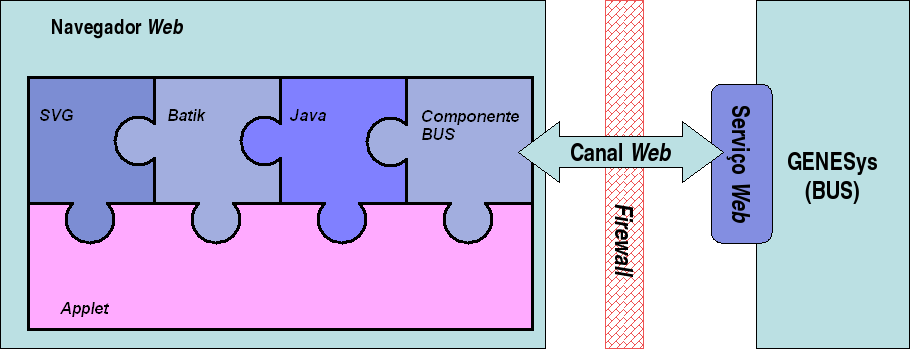
\includegraphics[width=0.86\textwidth]{puzzle}
    \caption{Architecture}
    \label{fig:arch}
\end{figure}

Loren ipsum dolor sit amet, consectetuer adipiscing elit. 
Praesent sit amet sem. Maecenas eleifend facilisis leo. Vestibulum et
mi. Aliquam posuere, ante non tristique consectetuer, dui elit
scelerisque augue, eu vehicula nibh nisi ac est. Nullam laoreet fermentum urna.

Duis eget diam. In est justo, tristique in, lacinia vel, feugiat eget,
quam. Pellentesque habitant morbi tristique senectus et netus et
malesuada fames ac turpis egestas. Fusce feugiat, elit ac placerat
fermentum, augue nisl ultricies eros, id fringilla enim sapien eu
felis. Vestibulum ante ipsum primis in faucibus orci luctus et
ultrices posuere cubilia Curae; Sed dolor mi, porttitor quis,
condimentum sed, luctus in. 

\subsection{Subsection Example} \label{sec:se322}

Suspendisse elementum sodales felis in Table~\ref{tab:example} is a 
floating table.

\begin{table}
  \caption{A table}
\begin{tabular}{|c|r@{.}lr@{.}lr@{.}l||r|}
	\hline
\multicolumn{8}{|c|}
	{\rule[-3mm]{0mm}{8mm}Iteration $k$ de $f(x_n)$} \\
\textbf{\em k}
	& \multicolumn{2}{c}{$x_1^k$}
	& \multicolumn{2}{c}{$x_2^k$}
	& \multicolumn{2}{c||}{$x_3^k$}
	& comments \\ \hline \hline
0   & -0&3                 & 0&6                 &  0&7   & - \\
1   &  0&47102965 & 0&04883157 & -0&53345964  & $\delta<\epsilon$ \\
2   &  0&49988691 & 0&00228830 & -0&52246185  & $\delta < \varepsilon$ \\
3   &  0&49999976 & 0&00005380 & -0&523656   &   $N$ \\
4   &  0&5                 & 0&00000307 & -0&52359743  & \\
\vdots	& \multicolumn{2}{c}{\vdots}
	& \multicolumn{2}{c}{$\ddots$}
	& \multicolumn{2}{c||}{\vdots}  & \\
7   &  0&5   & 0&0    & \textbf{-0}&\textbf{52359878}
		 & $\delta<10^{-8}$ \\ \hline
\end{tabular}
  \label{tab:example}
\end{table}

Loren ipsum dolor sit amet, consectetuer adipiscing elit. 
Praesent sit amet sem. Maecenas eleifend facilisis leo. Vestibulum et
mi. Aliquam posuere, ante non tristique consectetuer, dui elit
scelerisque augue, eu vehicula nibh nisi ac est. Suspendisse elementum
sodales felis. Nullam laoreet fermentum urna. 

Duis eget diam. In est justo, tristique in, lacinia vel, feugiat eget,
quam. Pellentesque habitant morbi tristique senectus et netus et
malesuada fames ac turpis egestas. Fusce feugiat, elit ac placerat
fermentum, augue nisl ultricies eros, id fringilla enim sapien eu
felis. Vestibulum ante ipsum primis in faucibus orci luctus et
ultrices posuere cubilia Curae; Sed dolor mi, porttitor quis,
condimentum sed, luctus in. 

\section{Section Example}

Loren ipsum dolor sit amet, consectetuer adipiscing elit. 
Praesent sit amet sem. Maecenas eleifend facilisis leo. Vestibulum et
mi. Aliquam posuere, ante non tristique consectetuer, dui elit
scelerisque augue, eu vehicula nibh nisi ac est. Suspendisse elementum
sodales felis. Nullam laoreet fermentum urna. 

\section{Summary}

Pellentesque habitant morbi tristique senectus et netus et
malesuada fames ac turpis egestas. Fusce feugiat, elit ac placerat
fermentum, augue nisl ultricies eros, id fringilla enim sapien eu
felis. Vestibulum ante ipsum primis in faucibus orci luctus et
ultrices posuere cubilia Curae; Sed dolor mi, porttitor quis,
condimentum sed, luctus in. 

%%%% Another chapter to force two pages in the index
%%%%
\chapter{Another chapter}

Integer nec quam. Sed fermentum. Nunc vitae leo. Etiam sit amet
quam. Nunc vestibulum massa in mauris. Duis eget nulla. 

\section{Section Example}

Fusce ultricies arcu eu nibh volutpat feugiat. Maecenas urna pede, 
commodo quis, porta eu, bibendum elementum, pede. 

\section{Section Example}

Sed eros massa, molestie eget, mattis non, rutrum ac, magna. 
Duis dui. Maecenas eget tortor ut dolor semper mattis. 
Maecenas auctor, tellus et ultricies tempor, elit
est placerat lacus, in posuere mauris lorem et arcu. 

\subsection{Subsection Example}

Nulla nec eros et pede vehicula aliquam. Aenean sodales pede vel
ante. Fusce sollicitudin sodales lacus. Maecenas justo mauris,
adipiscing vitae, ornare quis, convallis nec, eros. 

\subsection{Subsection Example}

Pellentesque pulvinar fringilla dolor. In sit amet pede. 
Proin orci justo, semper vel, vulputate quis, convallis
ac, nulla. Nulla at justo. Mauris feugiat dolor. 
Etiam posuere fermentum eros. Morbi nisl ipsum, tempus id, 
ornare quis, mattis id, dolor. Aenean molestie metus 
suscipit dolor. Aliquam id lectus sed
nisl lobortis rhoncus. Curabitur vitae diam sed sem aliquet
tempus. Sed scelerisque nisi nec sem.

\section{Section Example}

Sed eros massa, molestie eget, mattis non, rutrum ac, magna. 
Duis dui. Maecenas eget tortor ut dolor semper mattis. 
Maecenas auctor, tellus et ultricies tempor, elit
est placerat lacus, in posuere mauris lorem et arcu. 

\subsection{Subsection Example}

Nulla nec eros et pede vehicula aliquam. Aenean sodales pede vel
ante. Fusce sollicitudin sodales lacus. Maecenas justo mauris,
adipiscing vitae, ornare quis, convallis nec, eros. 

\subsection{Subsection Example}

Aliquam id lectus sed nisl lobortis rhoncus. 
Curabitur vitae diam sed sem aliquet tempus. Sed scelerisque 
nisi nec sem \textcite{khakipoor_linear_2023,liu_energy_2023}.

\section{Section Example}

Maecenas urna pede, commodo quis, porta eu, bibendum elementum, 
pede. Sed eros massa, molestie eget, mattis non, rutrum ac, 
magna. Duis dui. Maecenas eget tortor ut dolor semper mattis. 
Maecenas auctor, tellus et ultricies tempor, elit est placerat 
lacus, in posuere mauris lorem et arcu~\parencite{monopoli_exploiting_2023,zhang_carma_2023,chang_adas_2023, guo_rapidstream_2023}. 

\subsection{Subsection Example}

Nulla nec eros et pede vehicula aliquam. Aenean sodales pede vel
ante. Fusce sollicitudin sodales lacus. Maecenas justo mauris,
adipiscing vitae, ornare quis, convallis nec, eros. 

\subsection{Subsection Example}

Aliquam id lectus sed nisl lobortis rhoncus. 
Curabitur vitae diam sed sem aliquet tempus. Sed scelerisque 
nisi nec sem \textcite{khakipoor_linear_2023,liu_energy_2023} scelerisque.

Nulla nec eros et pede vehicula aliquam. Aenean sodales pede vel
ante. Fusce sollicitudin sodales lacus. Maecenas justo mauris,
adipiscing vitae, ornare quis, convallis nec, eros. Etiam laoreet
venenatis ipsum. In tellus odio, eleifend ac, ultrices vel, lobortis
sed, nibh. Fusce nunc augue, dictum non, pulvinar sed, consectetuer
eu, ipsum. Vivamus nec pede.  

%% Uncomment to see a listing example (see meic.cfg)
%%%% an example on how to include code
%%% ---------------------------------
\section{Listing example}

Pellentesque habitant morbi tristique senectus et netus et
malesuada fames ac turpis egestas. Fusce feugiat, elit ac placerat
fermentum, augue nisl ultricies eros, id fringilla enim sapien eu
felis.

\begin{lstlisting}[language=Python, caption=Python example, label=code:useless]
# Take the user's input
words = input("Enter the text to translate to pig latin: ")
print(f"You entered: {words}")

# Break apart the words into a list
words = words.split(' ')

# Use a list comprehension to translate words greater than or equal to 3 characters
translated_words = [(w[1:] + w[0] + "ay") for w in words if len(w) >= 3 ]

# Print each translated word
for word in translated_words:
    print(word)
\end{lstlisting}

Listing~\ref{code:useless} uis eget diam. In est justo, tristique in, lacinia vel, feugiat eget,
quam. Pellentesque habitant morbi tristique senectus et netus et
malesuada fames ac turpis egestas. Fusce feugiat, elit ac placerat
fermentum, augue nisl ultricies eros, id fringilla enim sapien eu
felis. Vestibulum ante ipsum primis in faucibus orci luctus et
ultrices posuere cubilia Curae; Sed dolor mi, porttitor quis,
condimentum sed, luctus in.

%%----------------------------------------
%% Final materials
%%----------------------------------------

%% Bibliography
\PrintBib

%% comment next 2 commands if numbered appendices are not used
\appendix
%% an example of appendix
\chapter{Lorem Ipsum} \label{ap1:Lorem}

After the conclusions and bibliographical references,
the text used to complete the dissertation is presented in this 
numbered annex. 

\section{What is \emph{Lorem Ipsum}?}

\emph{\textbf{Lorem Ipsum}} is simply dummy text of the printing and
typesetting industry. Lorem Ipsum has been the industry's standard
dummy text ever since the 1500s, when an unknown printer took a galley
of type and scrambled it to make a type specimen book. It has survived
not only five centuries, but also the leap into electronic
typesetting, remaining essentially unchanged. It was popularised in
the 1960s with the release of Letraset sheets containing Lorem Ipsum
passages, and more recently with desktop publishing software like
Aldus PageMaker including versions of Lorem Ipsum~\cite{kn:Lip08}. 

\section{Where does \emph{Lorem} come from?}

Contrary to popular belief, Lorem Ipsum is not simply random text. It
has roots in a piece of classical Latin literature from 45 BC, making
it over 2000 years old. Richard McClintock, a Latin professor at
Hampden-Sydney College in Virginia, looked up one of the more obscure
Latin words, consectetur, from a Lorem Ipsum passage, and going
through the cites of the word in classical literature, discovered the
undoubtable source. Lorem Ipsum comes from sections 1.10.32 and
1.10.33 of ``de Finibus Bonorum et Malorum'' (The Extremes of Good and
Evil) by Cicero, written in 45 BC. This book is a treatise on the
theory of ethics, very popular during the Renaissance. The first line
of Lorem Ipsum, ``Lorem ipsum dolor sit amet\ldots'', comes from a line in
section 1.10.32.

The standard chunk of Lorem Ipsum used since the 1500s is reproduced
below for those interested. Sections 1.10.32 and 1.10.33 from ``de
Finibus Bonorum et Malorum'' by Cicero are also reproduced in their
exact original form, accompanied by English versions from the 1914
translation by H. Rackham.

\section{Why is \emph{Lorem} used?}

It is a long established fact that a reader will be distracted by the
readable content of a page when looking at its layout. The point of
using Lorem Ipsum is that it has a more-or-less normal distribution of
letters, as opposed to using ``Content here, content here'', making it
look like readable English. Many desktop publishing packages and web
page editors now use Lorem Ipsum as their default model text, and a
search for ``lorem ipsum'' will uncover many web sites still in their
infancy. Various versions have evolved over the years, sometimes by
accident, sometimes on purpose (injected humour and the like). 

\section{Where can you find examples?}

There are many variations of passages of Lorem Ipsum available, but
the majority have suffered alteration in some form, by injected
humour, or randomised words which don't look even slightly
believable. If you are going to use a passage of Lorem Ipsum, you need
to be sure there isn't anything embarrassing hidden in the middle of
text. All the Lorem Ipsum generators on the Internet tend to repeat
predefined chunks as necessary, making this the first true generator
on the Internet. It uses a dictionary of over 200 Latin words,
combined with a handful of model sentence structures, to generate
Lorem Ipsum which looks reasonable. The generated Lorem Ipsum is
therefore always free from repetition, injected humour, or
non-characteristic words etc. 


\end{document}
